\documentclass[12pt]{article}

\usepackage{sbc-template}

\usepackage{graphicx,url}

\usepackage[brazil]{babel}   
%\usepackage[latin1]{inputenc}  
\usepackage[utf8]{inputenc}
% UTF-8 encoding is recommended by ShareLaTex

     
\sloppy

\title{Propuesta de un Sistema de e-Health usando reconocimiento de lenguaje natural desde un aplicativo móvil sobre un Sistema Cognitivo}

\author{Authors}
%\author{Christian Guevara, Carolina López, Denisse Calle, Iván Carrera\inst{1}}

\address{Institutions}
%\address{Facultad de Ingenier{\'i}a de Sistemas -- Escuela Polit{\'e}cnica Nacional (EPN)\\
%Ladr{\'o}n de Guevara E11-253. Quito -- Ecuador
%\email{\{christian.guevara,carolina.lopez,ivan.carrera\}@epn.edu.ec, \newline denisse@hmedic.com}
%}

\begin{document} 

\maketitle

\begin{abstract}
This work describes an e-Health system that will use a mobile app and a cognitive system trained with medical information to answer queries about health to prevent maternal death using a natural language. The requested information will be stored for a further analysis where, with anonymous geo-localization of users, factors can be assessed looking for trends in symptoms that affect a certain geographic area. Information will help Ministry of Public Health of Ecuador for the National Program for Prevention of Maternal and Neo-natal Death, as well as the Millenuim Objectives of the World Health Organization.
\end{abstract}
     
\begin{resumen} 
Este artículo describe un sistema de e-Health que usará una aplicación móvil y un sistema cognitivo entrenado con información médica para responder inquietudes de salud como mecanismo de prevención de la mortalidad materna utilizando un lenguaje natural. La información solicitada por el usuario y entregada por el sistema será almacenada para un posterior análisis en el que, geolocalizando anónimamente a los usuarios, se buscarán factores que muestren un incremento en síntomas manifiestos en una zona geográfica. La información contribuirá con el Ministerio de Salud Pública del Ecuador para el programa de prevención de mortalidad materna y neonatal, y también con los objetivos del milenio planteados por la Organización Mundial de la Salud.
\end{resumen}


\section{Introducción}
Actualmente, los sistemas computacionales cognitivos pueden imitar las capacidades del cerebro humano \cite{banavar2015watson}, permitiendo que puedan analizar e interpretar información. Uno de los sistemas cognitivos más utilizado en la actualidad es IBM Watson, disponible al público desde la plataforma IBM Bluemix \cite{watson2016}, donde los usuarios pueden crear instancias para realizar análisis sobre temas específicos. El desafío es lograr comunicación entre humano y computador a través de un lenguaje natural \cite{ibm2015}, para ofrecer resultados acorde a las necesidades de los usuarios, ampliando el acceso a la información.

El presente artículo propone la creación de un sistema de e-Health capaz de recibir preguntas médicas en lenguaje natural, a través de una interfaz móvil donde el ingreso de datos sea través de un cuadro de texto o de una grabación de voz. Se utilizará un conjunto de servicios web para recopilar información de las inquietudes de los usuarios ligada a la respuesta entregada por el sistema cognitivo. Esta información se análizará posteriormente para determinar las más frecuentes durante el embarazo y primeros meses de vida, buscando generar políticas públicas para disminuir el índice de mortalidad de madres y neonatos en el país.

En la Cumbre del Milenio realizada en 2000, 189 países miembros de las Naciones Unidas (NNUU) firmaron la Declaración del Milenio, que asume 8 objetivos a cumplir hasta el 2015 \cite{nnuu2000}. Entre sus objetivos relacionados a la Salud está “Mejorar la Salud Materna”, donde se plantea la meta de reducir la razón de mortalidad materna en 75\% entre 1990 y 2015. La mortalidad materna está definida por la Organización Mundial de la Salud (OMS) como la muerte de una mujer durante el embarazo, el parto o las 6 semanas después del parto \cite{oms2015b}.

%Durante la década de 1990 el Ministerio de Salud Pública del Ecuador (MSP) creó la Ley de Maternidad Gratuita y Atención a la Infancia. En el año 2008 se publica el Plan Nacional de Reducción Acelerada de la Mortalidad Materna y Neonatal. Finalmente en el 2014, se implementa la Gerencia Institucional para la Reducción Acelerada de Muerte Materna. \cite{msp2008b}

El 99\% de las muertes maternas corresponde a los países en desarrollo, que se vincula directamente con el acceso a servicios de salud y cobertura universal. % \cite{oms2015a}. %Ecuador ha logrado reducir la muerte materna en un 65,4\%, lo que no llega a la meta establecida, pero muestra un evidente progreso. La Norma para el Cuidado Obstétrico y Neonatal Esencial en el Sistema Nacional de Salud, publicada en el 2013, reporta que el 55\% de las causas de muerte materna pueden ser prevenibles \cite{msp2013}.
Entre los factores que impiden que las mujeres reciban o busquen atención durante el embarazo y el parto se encuentran la pobreza, la distancia hacia los servicios de salud, la falta de información, la inexistencia de servicios adecuados, las prácticas culturales, entre otros. Para mejorar la salud materna hay que identificar y eliminar los obstáculos al acceso a servicios de salud de calidad en todos los niveles del sistema sanitario \cite{oms2015c}

Con un buen uso y amplio acceso, la eSalud puede ser una herramienta estratégica al mejorar el acceso, ampliar la cobertura y aumentar la eficiencia financiera de los sistemas de atención de salud \cite{ops2014}. En Ecuador, según cifras del Instituto Nacional de Estadística y Censos (INEC), se reporta que el 48,5\% de ecuatorianos cuentan con un PC y el 24,3\% con un teléfono inteligente \cite{inec2014}. El sistema de e-Health deberá permitir realizar una debida capacitación y una constante vigilancia de los factores que afecten la salud de las mujeres embarazadas.

\section{Diseño}
\label{sec:diseno}

Se plantea el desarrollo de un sistema de e-Health para ofrecer una interfaz para realizar preguntas y obtener respuestas acerca de salud materna y neonatal. El sistema de e-Health usará un sistema cognitivo para obtener las respuestas a las preguntas ingresadas por los usuarios. La interacción con los usuarios se realizará por medio de un lenguaje natural. A su vez, la aplicación móvil estará conectada al sistema cognitivo a través de un conjunto de servicios web. Este back-end de servicios se usará para la recolección y procesamiento de las preguntas y respuestas para obtener información sobre factores comunes que incidan en la salud materna y neonatal dentro de un área geográfica específica.

El sistema descrito consta de tres etapas: la aplicación móvil, el back-end de servicios web y el sistema cognitivo. Para la construcción, alojamiento y ejecución de los diferentes componentes necesarios, en la Figura \ref{fig:arquitectura} se plantea el diagrama de arquitectura del sistema. Los componentes se describen a continuación:

\begin{figure}[ht]
\centering
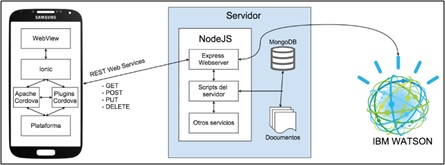
\includegraphics[width=.75\textwidth]{model.jpg}
\caption{Diagrama de Arquitectura del Sistema}
\label{fig:arquitectura}
\end{figure}

%Entre los servicios de IBM Watson disponibles al público está \emph{Retrieve and Rank}, que recibe información estructurada para su procesamiento y posteriormente utilizada en el entrenamiento del modelo. El modelo de aprendizaje de este servicio se basa en un conjunto de preguntas, sus posibles respuestas y su respectivo nivel de asertividad. A través de dicho modelo se ofrecen los resultados mejor puntuados a las inquietudes planteadas por los usuarios \cite{watson2016}. 

%Para la implementación de los componentes del sistema, especificados en la arquitectura, se usará el mismo lenguaje de programación, en este caso JavaScript. Esto permite una fácil interacción entre los componentes, además de simplificar el desarrollo a un solo lenguaje de programación.

\begin{itemize}
\item \textbf{Aplicación Móvil.} Es la interfaz de los usuarios para realizar las consultas médicas. Los usuarios tienen la facilidad de ingresar consultas con texto o voz en lenguaje español, usando una librería \emph{speech-to-text} que traduce el mensaje de voz en texto. La aplicación móvil se desarrolla en un solo lenguaje y puede ser instalada en sistemas Android e iOS. Esta aplicación se desarrolla sobre el framework \emph{Apache Cordova} en conjunto con \emph{Ionic} y \emph{AngularJS} para el manejo de la interfaz y la interacción entre sus componentes.\\

\item \textbf{Back-end de Servicios.} El middleware entre la aplicación móvil y el sistema cognitivo para la publicación de servicios web y almacenamiento de información para análisis posterior. La información recopilada será: la ubicación del usuario, la pregunta realizada y las respuestas obtenidas. Esta información se almacenará en una base de datos no relacional, debido a que las respuestas obtenidas y las preguntas realizadas no tienen un formato definido. El entorno de ejecución es \emph{NodeJS}, donde se ejecutará un framework web, y sobre él estarán disponibles los servicios utilizados en la comunicación y paso de información entre componentes.\\

\item \textbf{Sistema Cognitivo.} El conjunto de servicios de nube IBM Bluemix tiene la capacidad de crear instancias con todas las funcionalidades del sistema cognitivo Watson, restringidas a un tema específico. La instancia para el sistema será entrenada con información médica en el ámbito de mortalidad materna y neonatal. El sistema cognitivo se encarga de procesar e interpretar la información médica a través del servicio \emph{Retrieve and Rank} para generar un modelo de aprendizaje basado en resultados de acuerdo con su nivel de asertividad \cite{ibm2015}. Sus algoritmos analizan la pregunta y buscan posibles respuestas dentro del modelo generado, mientras se evalúan y se les asigna un puntaje \cite{ibm2013}.

\end{itemize}

%El diseño prevé que el sistema congnitivo vaya adquiriendo mayor conocimiento sobre temas específicos y amplíe el rango de preguntas que se le pueden realizar.

\section{Implementación}

Se implementó un prototipo de aplicación móvil capaz de recibir la pregunta del usuario en texto y enviarla hacia el servicio \emph{Retrieve and Rank} de IBM Watson. Se cargaron datos en el servicio y se entrenó un modelo de aprendizaje basado en resultados conocidos y relevantes. El servicio aprovecha ese modelo para proporcionar resultados mejorados \cite{ibm2016} a los usuarios del prototipo móvil en función de sus inquietudes. Los datos fueron recopilados manualmente en base a las preguntas más comunes en el área de la salud materna y neonatal, estas preguntas fueron puntuadas y enviadas al servicio \emph{Retrieve and Rank} para entrenar el modelo de aprendizaje. Se utilizaron 57 preguntas, cada pregunta con 3 respuestas y cada respuesta con su respectivo porcentaje de asertividad.

\emph{Retrieve and Rank} hace uso del motor \emph{Apache Solr} para facilitar las búsquedas en grandes conjuntos de datos \cite{ibm2016}. La configuración usada como modelo para datos estructurados en documentos generados previamente es la usada en el demo del servicio \cite{ibm2015rr}. Para la comunicación entre el prototipo de aplicación y el sistema cognitivo se usa REST como protocolo de transferencia con tramas JSON para la extracción de datos. En el prototipo de la aplicación móvil se puede ingresar la pregunta a través de texto y recibir un conjunto de respuestas escogidas por el sistema cognitvo.

%\begin{figure}[ht]
%\centering
%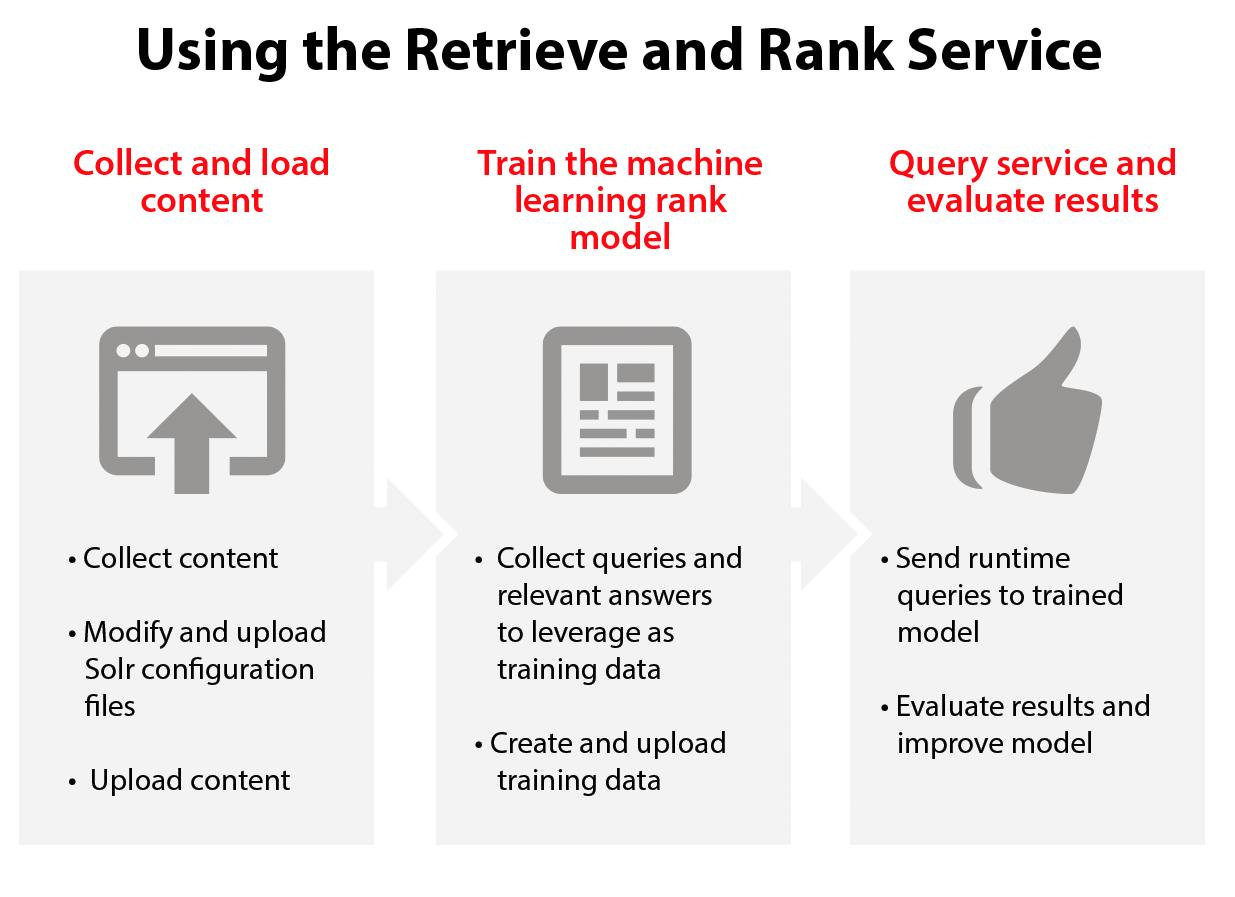
\includegraphics[width=.75\textwidth]{retrieve.jpg}
%\caption{Diagrama de Arquitectura}
%\label{fig:retrieve}
%\end{figure}

\section{Conclusiones y Trabajos Futuros}

Es necesario mencionar que el Sistema de e-Health, si bien responderá a inquietudes de salud materna y neonatal, no pretende reemplazar el cuidado y control médico oportuno. El sistema no podrá reemplazar la acción de un médico, sino que busca que los usuarios tengan un mayor conocimiento y acceso a buenas prácticas y cuidados en salud materna.

Aún se debe completar la implementación del middleware de comunicación entre la aplicación móvil y el sistema cognitivo descrito en la Figura \ref{fig:arquitectura}. Este middleware estará en la capacidad de almacenar la información de las preguntas realizadas por el usuario y de las respuestas obtenidas del servicio del sistema cognitivo.

Se deberá usar la información ofrecida por el Ministerio de Salud del Ecuador para generar el corpus y entrenar a la instancia de sistema cognitivo. %Dicha instancia se especializará en información de muertes maternas y de neonatos en el Ecuador; para en un futuro con la información recolectada y almacenada en el middleware, se plantea realizar un análisis de datos que permita determinar factores y reducir el índice de muertes en el país.
Un mayor acceso a información sobre servicios de salud, a través de este sistema de e-Health, apoyará a conseguir el objetivo mundial y local de la reducción de la mortalidad materna.

%\begin{figure}[ht]
%\centering
%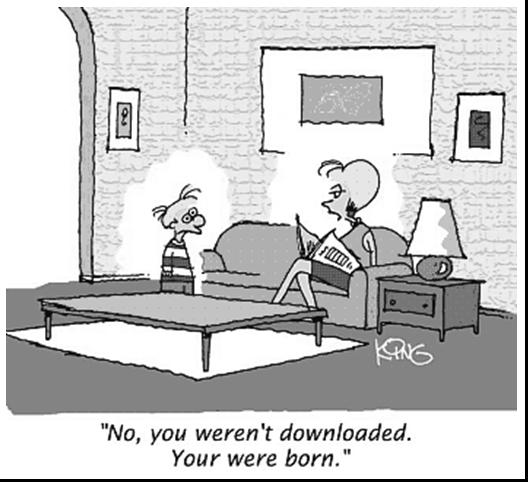
\includegraphics[width=.5\textwidth]{fig1.jpg}
%\caption{A typical figure}
%\label{fig:exampleFig1}
%\end{figure}
%
%\begin{figure}[ht]
%\centering
%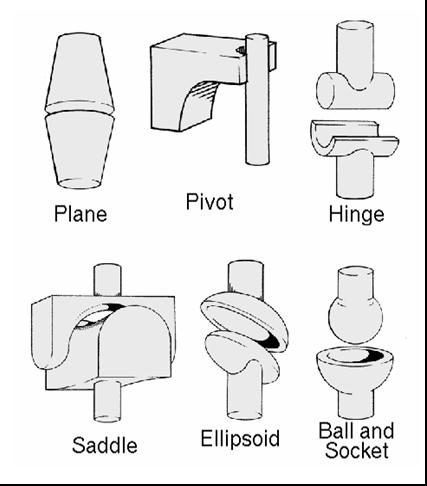
\includegraphics[width=.3\textwidth]{fig2.jpg}
%\caption{This figure is an example of a figure caption taking more than one
  %line and justified considering margins mentioned in Section~\ref{sec:figs}.}
%\label{fig:exampleFig2}
%\end{figure}

%In tables, try to avoid the use of colored or shaded backgrounds, and avoid
%thick, doubled, or unnecessary framing lines. When reporting empirical data,
%do not use more decimal digits than warranted by their precision and
%reproducibility. Table caption must be placed before the table (see Table 1)
%and the font used must also be Helvetica, 10 point, boldface, with 6 points of
%space before and after each caption.

%\begin{table}[ht]
%\centering
%\caption{Variables to be considered on the evaluation of interaction
%  techniques}
%\label{tab:exTable1}
%\smallskip
%\begin{tabular}{|l|c|c|}
%\hline
%& Value 1 & Value 2\\[0.5ex]
%\hline
%&&\\[-2ex]
%Case 1 & 1.0 $\pm$ 0.1 & 1.75$\times$10$^{-5}$ $\pm$ 5$\times$10$^{-7}$\\[0.5ex]
%\hline
%&&\\[-2ex]
%Case 2 & 0.003(1) & 100.0\\[0.5ex]
%\hline
%\end{tabular}
%\end{table}

\bibliographystyle{sbc}
\bibliography{sbc-template}

\end{document}
